% Created 2019-07-16 Tue 17:20
% Intended LaTeX compiler: pdflatex
\documentclass[11pt]{article}
\usepackage[latin1]{inputenc}
\usepackage[T1]{fontenc}
\usepackage{graphicx}
\usepackage{grffile}
\usepackage{longtable}
\usepackage{wrapfig}
\usepackage{rotating}
\usepackage[normalem]{ulem}
\usepackage{amsmath}
\usepackage{textcomp}
\usepackage{amssymb}
\usepackage{capt-of}
\usepackage{hyperref}
\author{Nicol�s Luarte}
\date{\today}
\title{Francisca}
\hypersetup{
 pdfauthor={Nicol�s Luarte},
 pdftitle={Francisca},
 pdfkeywords={},
 pdfsubject={},
 pdfcreator={Emacs 25.2.2 (Org mode 9.2.4)}, 
 pdflang={English}}
\begin{document}

\maketitle
\tableofcontents

\section{Calentamientos}
\label{sec:orgc0780ef}
\begin{center}
\begin{tabular}{lr}
Ejercicio & Protocolo\\
Extensiones de cuadriceps & 3x25\\
Buenos d�as sentada & 3x12\\
Fortalecimiento de psoas & 3x10\\
 & \\
\end{tabular}
\end{center}
\section{Ciclos}
\label{sec:org4225bc6}
\begin{center}
\begin{tabular}{lll}
Ejercicio & Protocolo & Bloque\\
\hline
Sentadilla de competencia & x5@8, 10\%, 5x5 & A\\
Banca de competencia & x6@8, 10\%, 5x6 & A\\
Press banca pies arriba (agarre cerrado) & x6@8, 15\%, 5x6 & A\\
\hline
Press banca agarre cerrado & x7@8, 10\%, 4x6 & B\\
Peso muerto convencional & x3@8, 10\%, 2x3 & B\\
Peso muerto sumo & x3@8, 10\%, 2x3 & B\\
\hline
\end{tabular}
\end{center}
\section{Comentarios t�cnicos}
\label{sec:orgac21eed}
\subsection{01/07/2019, ciclo 1, bloque a}
\label{sec:orga359e1a}
\subsubsection{Sentadilla de competencia}
\label{sec:org6a8bd7f}
\begin{enumerate}
\item Juntar un poquito más los pies
\item Reducir el ángulo de las punteras de los pies
\item Concentrarse en mantener las rodilas adelante
\item Reducir la velocidad de descenso
\item Pensar en llevar las rodillas hacia adelante
\item Realizar todo los sets luego del drop, con bandas alrededor de las
piernas, a altura de las rodillas
\end{enumerate}
\subsubsection{Banca de competencia}
\label{sec:orgc3cf40c}
\begin{enumerate}
\item Pausa activa, piensa que hay un huevo en tú pecho y no lo puedes
reventar
\item Retracción escapular, piensa que tienes que apretar una moneda que
te ponen en tú espalda con los hombros
\end{enumerate}
\subsubsection{Press banca pies arriba}
\label{sec:org149063c}
\begin{enumerate}
\item Mismos comentarios que para press banca
\end{enumerate}
\subsection{02/07/2019, ciclo 1, bloque b}
\label{sec:org087e3bc}
\subsubsection{Press banca agarre cerrado}
\label{sec:org220590c}
\begin{enumerate}
\item Centrarse en pensar que tienes un huevo en el pecho y por lo tanto
debes tener cuidado de no romperlo al bajar la barra
\item Baja un poco mas lento la barra
\end{enumerate}
\subsubsection{Peso muerto convencional}
\label{sec:org0d2d95e}
\begin{enumerate}
\item Debes tomar mas aire por tú boca, llevarlo a tu estomago, inflarlo
y luego apretar los abdominales hacia abajo
\item El bloqueo debe ser súper agresivo y rápido, toma la costumbre
desde el primer calentamiento, bloquear caderas rápido
\end{enumerate}
\subsubsection{Peso muerto sumo}
\label{sec:orgc44a00f}
\begin{enumerate}
\item Por ahora, solo trabajar en ir aumentando la apertura de las rodillas
\end{enumerate}
\subsection{04/07/2019, ciclo 1, bloque a}
\label{sec:org59a5396}
\subsubsection{Sentadilla de competencia}
\label{sec:orga066254}
\begin{enumerate}
\item Juntar un poquito más los pies
\item Reducir el ángulo de las punteras de los pies
\item Concentrarse en mantener las rodilas adelante
\item Reducir la velocidad de descenso
\item Pensar en llevar las rodillas hacia adelante
\item Realizar todo los sets luego del drop, con bandas alrededor de las
piernas, a altura de las rodillas
\item Bajar levemente los codos y hacer retracción escapular antes de
sacar la barra del rack, manteniendola durante todo el movimiento
\item Hacer mas exagerada la tomada de aire, y hacer también antes de
sacar la barra
\end{enumerate}
\subsubsection{Banca de competencia}
\label{sec:org49bc4e2}
\begin{enumerate}
\item Pausa activa, piensa que hay un huevo en tú pecho y no lo puedes
reventar
\item Retracción escapular, piensa que tienes que apretar una moneda que
te ponen en tú espalda con los hombros
\item Evitar ese rebote que haces para sacar la barra del pecho, recuerda
que la barra apenas debe tocar el pecho y luego salir de ahí
\item Piensa es llevar el pecho hacia la barra, en vez de la barra hacia
el pecho, con eso busco que exageres sacar el pecho mientras haces
la banca
\end{enumerate}
\subsubsection{Press banca pies arriba}
\label{sec:orgc5900ee}
\begin{enumerate}
\item Mismos comentarios que para press banca
\end{enumerate}
\subsection{06/07/2019, ciclo 1, bloque b}
\label{sec:org5182191}
\subsubsection{Press banca agarre cerrado}
\label{sec:orgd4272f2}
\begin{enumerate}
\item Centrarse en pensar que tienes un huevo en el pecho y por lo tanto
debes tener cuidado de no romperlo al bajar la barra
\item Baja un poco mas lento la barra
\item Cuidar de hacer la pausa reglamentaria
\item Mejoraste bastante el arco y la tocada en el pecho, revisa tu vídeo
para tomar nota mental para la siguiente sesión de banca, este es
un buen hábito cúando te salga bien un levantamiento revisalo,
fijandose y recordando las sensaciones y claves mentales que usaste
\end{enumerate}
\subsubsection{Peso muerto convencional}
\label{sec:orge466762}
\begin{enumerate}
\item Debes tomar mas aire por tú boca, llevarlo a tu estomago, inflarlo
y luego apretar los abdominales hacia abajo <- esto es
tremendamente fundamental sobretodo en peso muerto, piensa es tomar
todo el aire el gym y apretar como roca los abdominales
\item Busca ser paciente en el peso muerto. Ser paciente significa
principalmente dos cosas (a) debe estar todo en posici�n antes de
iniciar el levantamiento y por lo mismo evita rodar la barra y
bajar y volver a subir las cadera, (b) busca que las caderas queden
"altas" si bien puede se vea "feo" así es como se levanta
más. Cuando todo este en perfecta posici�n empiezas a tensar la
barra de a poquito hasta que este apunto de levantarse, aguantas un
segundo así y vas con todo para arriba
\end{enumerate}
\subsubsection{Peso muerto sumo}
\label{sec:orgd15eabf}
\begin{enumerate}
\item Por ahora, solo trabajar en ir aumentando la apertura de las rodillas
\end{enumerate}
\subsection{11/07/2019, ciclo 1, bloque a}
\label{sec:org0c7bf62}
\subsubsection{Sentadilla de competencia}
\label{sec:org4d85432}
\begin{itemize}
\item Abrir la postura un poco m�s (hasta d�nde sea c�modo)
\item Reducir la velocidad de descenso, debes contar m�nimo 3 missisipis
mientras vas descendiendo antes de llegar a profundidad
\item Realizar 3 sets de 25-40 repeticiones en la extensi�n de cuadriceps,
usando poco peso
\item Tratar de controlar lo mejor posible la subida, aunque eso disminuya
la velocidad, buscando dejar las rodillas en posici�n
\item Usar bandas en las rodillas para todas las variantes de sentadilla
al momento del volumen
\end{itemize}
\subsubsection{Banca de competencia}
\label{sec:orgf9b1b11}
\begin{itemize}
\item Por ahora concentrarse en mantener la tensi�n tocando el pecho y
hacer fuerza con la piernas para empujarte hacia atr�s durante todo
el levantamiento
\end{itemize}
\subsection{13/07/2019, ciclo 1, bloque b}
\label{sec:org3c4e3a2}
\textbf{CONSIDERAR NUEVO PROTOCOLO DE CALENTAMIENTO, SE DEBE REALIZAR ANTES DE
 CADA SESI�N}
\subsubsection{Press banca agarre cerrado}
\label{sec:org9c3cb80}
\begin{itemize}
\item Cuidar que la barra no se hunda en el pecho
\item Seguir reforzando la pausa activa, esto es, que la barra apenas
toque el pecho, siempre en tensi�n
\end{itemize}
\subsubsection{Peso muerto convencional}
\label{sec:orgd2e066c}
\begin{itemize}
\item Practicar tensar la barra ("sacarle el slack")
\item Mantener la tensi�n constante por 1-2 segundos, luego levantar sin
volver a perder tensi�n
\end{itemize}
\subsubsection{Peso muerto sumo}
\label{sec:org4cbe088}
\begin{itemize}
\item Aplicar los mismos comentarios que para peso muerto convencional
\end{itemize}
\subsection{15/07/2019, ciclo 1, bloque a}
\label{sec:orged05758}
\subsubsection{Sentadilla de competencia}
\label{sec:org1adaa63}
\begin{itemize}
\item De aqu� en adelante utilizar la postura con el torso mas inclinado que
lograste en esta sesi�n
\item Bajar un poquito menos justo hasta despu�s de paralelo
\item Reducir la velocidad, que el descenso sea suave y controlado
\end{itemize}
\subsubsection{Banca de competencia}
\label{sec:org2ee7f30}
\begin{itemize}
\item Concentrarse en hacer tensi�n con las piernas durante todo el movimiento
\end{itemize}
\section{Registro de progreso}
\label{sec:orgd6b2ac6}
\subsection{Ciclo 1}
\label{sec:org8be6b27}
\begin{center}
\label{tab:org75082d4}
\begin{tabular}{lrrl}
Ejercicio & RPE & Peso & Fecha\\
\hline
Sentadilla de competencia & 8 & 65 & 01/07/2019\\
Press banca de competencia & 8 & 38 & 01/07/2019\\
Press banca pies arriba & 10 & 38 & 01/07/2019\\
Press banca agarre cerrado & 8 & 34 & 02/07/2019\\
Peso muerto convencional & 8 & 88 & 02/07/2019\\
Peso muerto sumo & 8 & 70 & 02/07/2019\\
Sentadilla de competencia & 8 & 65 & 04/07/2019\\
Press banca de competencia & 8 & 43 & 04/07/2019\\
Press banca pies arriba & 8 & 34 & 04/07/2019\\
Peso muerto convencional & 8 & 93 & 06/07/2019\\
Peso muerto sumo & 8 & 60 & 06/07/2019\\
Press banca agarre cerrado & 8 & 34 & 06/07/2019\\
Sentadilla de competencia & 8 & 70 & 11/07/2019\\
Press banca de competencia & 8 & 43 & 11/07/2019\\
Press banca pies agarre cerrado & 8 & 34 & 11/07/2019\\
Press banca agarre cerrado & 8 & 34 & 13/07/2019\\
Peso muerto convencional & 8 & 93 & 13/07/2019\\
Peso muerto sumo & 8 & 60 & 13/07/2019\\
Sentadilla de competencia & 8 & 60 & 15/07/2019\\
Press banca de competencia & 8 & 38 & 15/07/2019\\
Press banca agarre cerrado & 8 & 34 & 15/07/2019\\
 &  &  & \\
\end{tabular}
\end{center}
\subsection{Plots}
\label{sec:orgfeba7d7}
\subsubsection{Ciclo 1}
\label{sec:orgc447bea}
\begin{center}
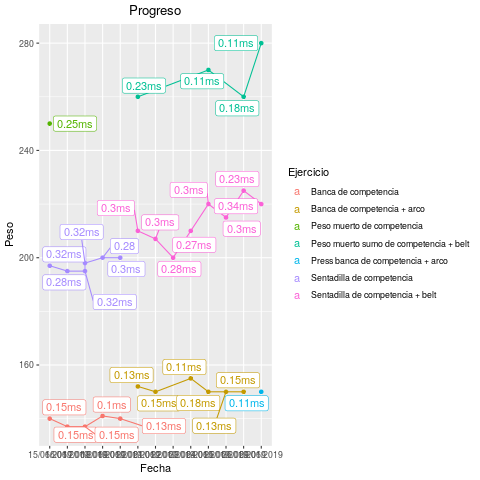
\includegraphics[width=.9\linewidth]{tmp.png}
\end{center}
\end{document}
